\documentclass[usenames,dvipsnames,t]{beamer}

\usepackage[english]{babel}
\usepackage[utf8]{inputenc}
\usepackage{amsmath,amsthm, amssymb, latexsym}
\usepackage{amssymb}
\usepackage{color}
\usepackage{tikz}
\usepackage{standalone}
\usepackage{minted}
%\usepackage{lmodern}
\usepackage{fontawesome}
\usepackage{setspace}

\definecolor{DarkGray}{RGB}{5, 66, 81}
\definecolor{DarkerGray}{RGB}{3, 22, 27}

\usemintedstyle{native}

\usetikzlibrary{shapes.arrows, positioning, arrows, decorations.pathreplacing,
angles, quotes, decorations.pathmorphing}
\tikzset{
    ultra thick/.style={line width=3pt}
}

\usecolortheme[dark,accent=cyan]{solarized}
\beamertemplatenavigationsymbolsempty
\setbeamerfont{block title}{size=\Large}
\usepackage[orientation=landscape,size=a1,scale=1.4]{beamerposter}
\newcommand{\R}{\mathbb{R}}

\renewcommand{\arraystretch}{1.2}

\addtobeamertemplate{block begin}{%
  \setlength{\textwidth}{.5\textwidth}%
}{}

\addtobeamertemplate{block alerted begin}{%
  \setlength{\textwidth}{.5\textwidth}%
}{}

\addtobeamertemplate{block example begin}{%
  \setlength{\textwidth}{.5\textwidth}%
}{}
%%%%%%%%%%%%%%%%%%%%%%%%%%%%%%%%%%%%%%%%%%%%%%%%%%%%%%%%%%%%%%%%%%%%%%%%%%%%%%%
\begin{document}

%%%%%%%%%%%%%%%%%%%%%%%%%%%%%%%%TITLE%%%%%%%%%%%%%%%%%%%%%%%%%%%%%%%%%%%%%%%%%%%
\begin{columns}
    % \begin{column}{.1\linewidth}
    % \end{column}
    \begin{column}{.55\linewidth}
    \vspace{1.5cm}

    \centering
    \textcolor{orange}{\fontsize{110}{120} \selectfont THE POWER OF MEMORY}
    \vspace{0.7cm}

    \Large\textcolor{orange}{In interactions both social and biological is memory
    size advantageous?}
    \end{column}
    \begin{column}{.2\linewidth}
        
        \begin{center}
            \includestandalone[width=.75\textwidth]{static/matrix}
        \end{center}
        \end{column}
    \begin{column}{.23\linewidth}

        \includestandalone[width=\textwidth]{static/memory_one}
    \end{column}
    \begin{column}{.02\linewidth}
    \end{column}
\end{columns}
% %%%%%%%%%%%%%%%%%%%%%%%%%%%%%%%%FIRST ROW%%%%%%%%%%%%%%%%%%%%%%%%%%%%%%%%%%%%%%%
\begin{columns}
    \begin{column}{.2\linewidth}
        \vspace{-.9cm}
        \begin{center}
            \includestandalone[width=.8\textwidth]{static/states}
        \end{center}
    \end{column}
    \begin{column}{.1\linewidth}
        \vspace{3.5cm}

            \includestandalone[width=.5\textwidth]{static/arrow}
    \end{column}
    \begin{column}{.25\linewidth}
        \vspace{1.5cm}

        \hspace{-2cm}\normalsize{
\(
\left[\begin{matrix}p_{1} q_{1} & p_{1} \left(- q_{1} + 1\right) & q_{1} \left(- p_{1} + 1\right) & \left(- p_{1} + 1\right) \left(- q_{1} + 1\right)\\
p_{2} q_{3} & p_{2} \left(- q_{3} + 1\right) & q_{3} \left(- p_{2} + 1\right) & \left(- p_{2} + 1\right) \left(- q_{3} + 1\right)\\
p_{3} q_{2} & p_{3} \left(- q_{2} + 1\right) & q_{2} \left(- p_{3} + 1\right) & \left(- p_{3} + 1\right) \left(- q_{2} + 1\right)\\
p_{4} q_{4} & p_{4} \left(- q_{4} + 1\right) & q_{4} \left(- p_{4} + 1\right) & \left(- p_{4} + 1\right) \left(- q_{4} + 1\right)\end{matrix}\right]
\)
} 
    \end{column}
    \begin{column}{.1\linewidth}
        \vspace{1.5cm}

        \includestandalone[width=.6\textwidth]{static/trident_arrow}
    \end{column}
    \begin{column}{.35\linewidth}
        \vspace{1cm}

        \small{
            W. H. Press and F. J. Dyson. \textbf{Iterated Prisoner’s
            Dilemma contains strategies that dominate any evolutionary opponent}
            PNAS 2012. Introducing the zero determinant strategies:
            \[p ^ * \rightarrow \text{ manipulates } \rightarrow q\]
        }
        \vspace{1cm}

        \small{
        This work considers an optimisation approach to identify:
        \[ p ^ * \rightarrow \text{ best response } \rightarrow q\]
            }
        % \small{
        %  \[\max_q: u_q(p) = \frac{\frac{1}{2}\enspace p  Q  p^T + c^T p + a}
        %           {\frac{1}{2}\enspace  p  \bar{Q}  p^T + \bar{c}^T  p + \bar{a}}\]
        %     }
    \end{column}
    \begin{column}{.2\linewidth}
    \end{column}
\end{columns}
\vspace{0.7cm}

\hrule height 5pt
%%%%%%%%%%%%%%%%%%%%%%%%%%%%%%%%SECOND ROW%%%%%%%%%%%%%%%%%%%%%%%%%%%%%%%%%%%%%%
\begin{columns}
    \begin{column}{.8\linewidth}
        \begin{center}
            \textcolor{orange}{\Large{PURELY RANDOM STRATEGIES \(p=(p, p, p, p)\)}}
        \end{center}
    \end{column}
    \begin{column}{.2\linewidth}
        \begin{center}
            \textcolor{orange}{\Large{RESULTS}}
        \end{center}
    \end{column}
\end{columns}

\begin{columns}
    \begin{column}{.4\linewidth}
        \centering
        \textcolor{solarizedOrange}{\large{AGAINST A SINGLE OPPONENT}}

        \begin{minipage}{50cm}
        \begin{block}
            
            \[p^* = \text{argmax}(u_q(p)), \ p \in S_q,\]
            \vspace{0.3cm}

            \small{
            where the set \(S_q\) is defined as,}
        
            \[S_q = \left \{0, p_{\pm}, 1 \left | \begin{array}{l} 0 < p_{\pm} < 1,
            \\ p_{\pm} \neq \frac{-d_0}{d_1} \end{array} \right. \right\}\]
        \end{block}
    \end{minipage}
    
    \includestandalone[width=.3\textwidth]{static/single_opponent}
    \end{column}
    \begin{column}{.4\linewidth}
        \centering
        \textcolor{solarizedOrange}{\large{AGAINST MULTIPLE OPPONENTS}}

        \begin{minipage}{50cm}
            \begin{block}

            \[p^* = \text{argmax}(\displaystyle \sum_{i=1} ^ {N} {u_q}^{(i)} (p)), \ p \in S_{q(i)},\]
            \vspace{0.3cm}

            \small{
            where the set \(S_{q(i)}\) is defined as:}

            \[ S_{q(i)} =  \overset{2N}{\underset{\lambda_i \neq \frac{do_i}{d1_i}}{\underset{i=1}{u}}} \lambda_i \cup \{0, 1\} \]
             \vspace{0.3cm}

            Note the size of candidate solutions is \( 1 \leq|S_{q(i)}| \leq 2N + 2\).
            \end{block}
        \end{minipage}

        \includestandalone[width=.3\textwidth]{static/multiple_opponents}
    \end{column}
    \begin{column}{.2\linewidth}
        \begin{enumerate}
            \item The first
            \item The second
            \item The third
        \end{enumerate}

        \begin{center}
            \textcolor{orange}{\Large{FUTURE WORK}}
        \end{center}
    \begin{center}
        \includestandalone[width=.5\textwidth]{static/resultant}
    \end{center}
    \end{column}
\end{columns}
% %%%%%%%%%%%%%%%%%%%%%%%%%%%%%%%%%%%THIRD ROW%%%%%%%%%%%%%%%%%%%%%%%%%%%%%%%%%%
\begin{columns}
    \begin{column}{.2\linewidth}
        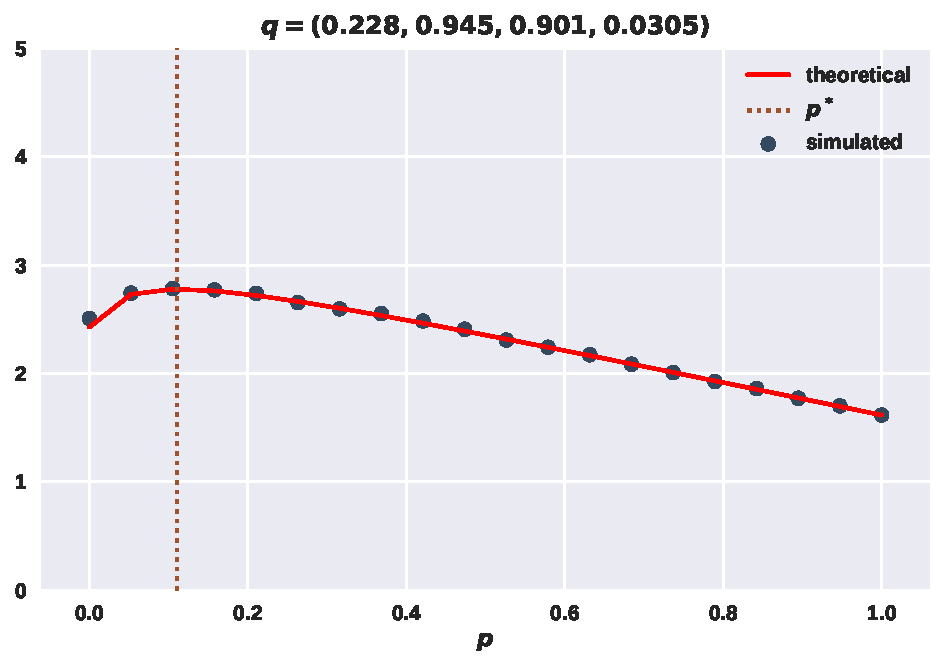
\includegraphics[width=\textwidth]{static/plot_one}
    \end{column}
    \begin{column}{.2\linewidth}
        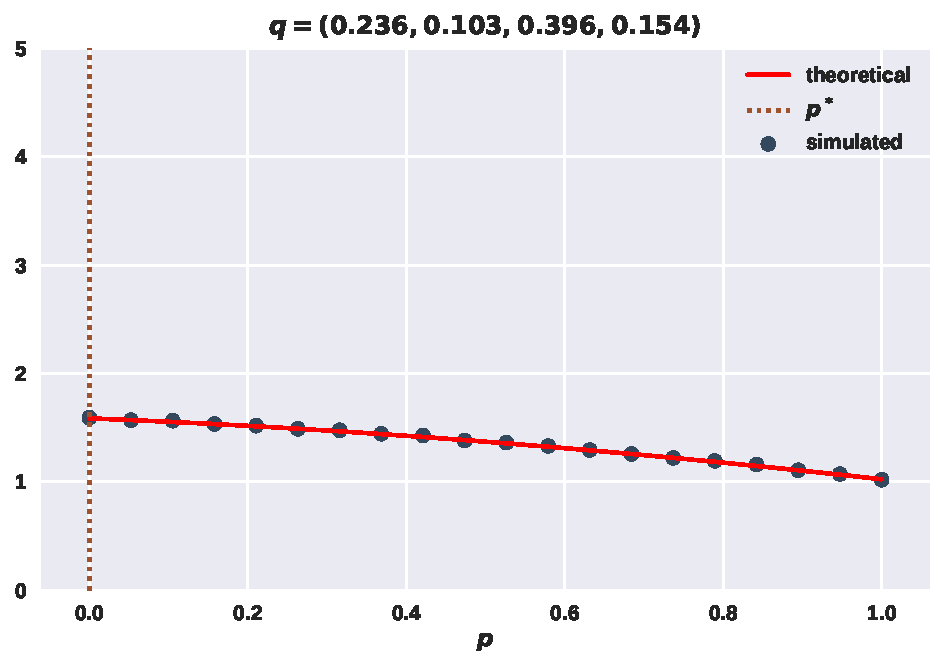
\includegraphics[width=\textwidth]{static/plot_two}
    \end{column}
    \begin{column}{.2\linewidth}
        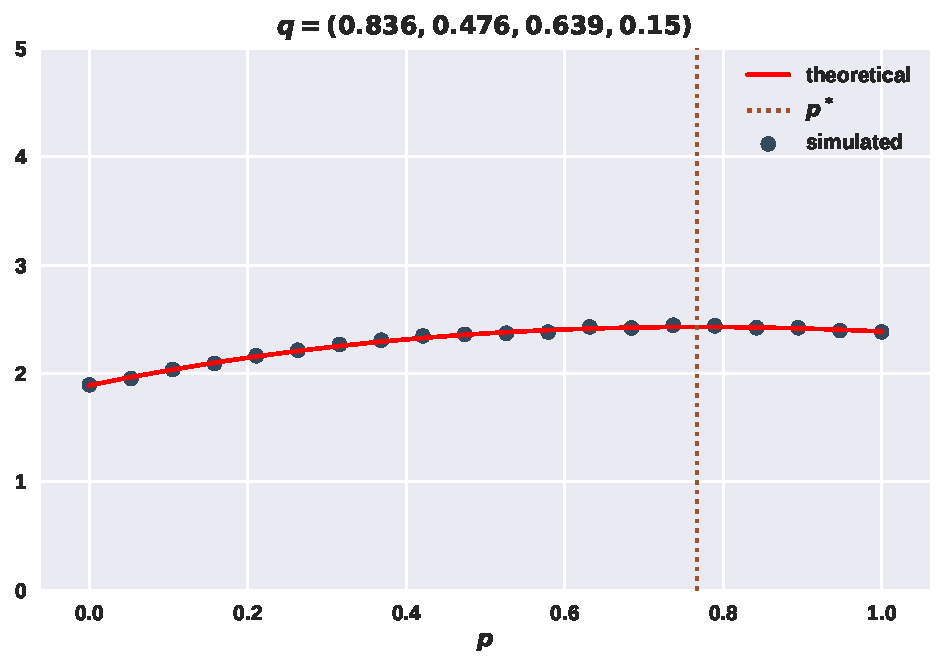
\includegraphics[width=\textwidth]{static/plot_three}
    \end{column}
    \begin{column}{.2\linewidth}
        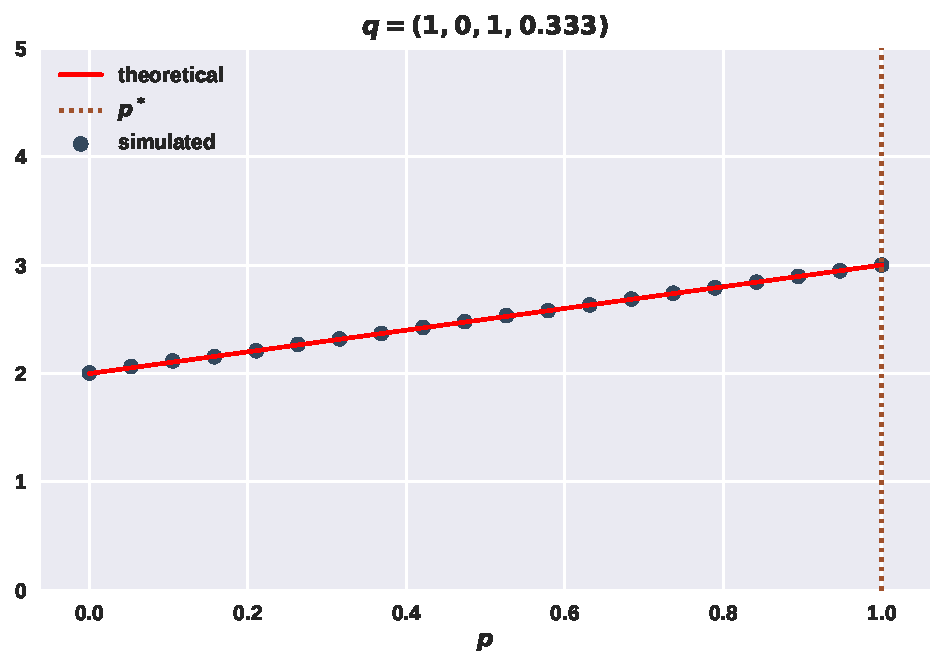
\includegraphics[width=\textwidth]{static/plot_four}
    \end{column}
    \begin{column}{.2\linewidth}
        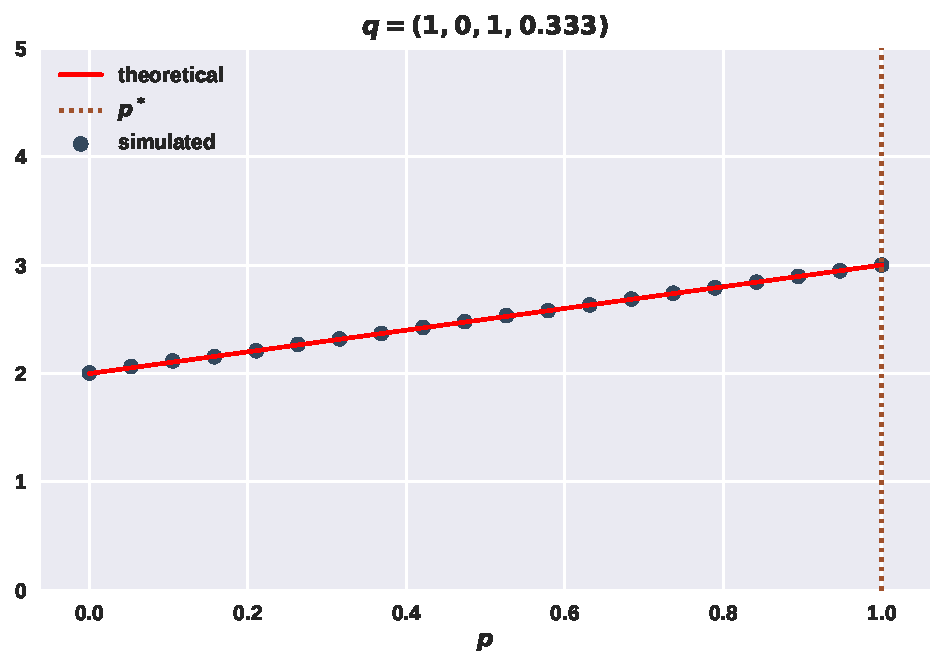
\includegraphics[width=\textwidth]{static/plot_four}
    \end{column}
\end{columns}
\vspace{1cm}

\hrule height 5pt
%%%%%%%%%%%%%%%%%%%%%%%%%%%%%%%%%%%%%INFO%%%%%%%%%%%%%%%%%%%%%%%%%%%%%%%%%%%%%%%
\begin{columns}
    \begin{column}{.8\linewidth}
        \hspace{1cm}
     \textbf{ \faTwitter \ NikoletaGlyn \hspace{2cm} In case you missed me: \url{nikoleta-v3.github.io/blog/2017/08/23/grudges-war-GoT.html} \hspace{2cm} \faGithub \ Nikoleta-v3}
     \end{column}
\end{columns}
\end{document}
